\documentclass[12pt]{extarticle}
\setlength{\columnsep}{2.5em}
\usepackage[margin=15pt,a4paper,]{geometry}

\usepackage{tasks}
%\usepackage[margin=45pt,a4paper,]{geometry}
%\usepackage[hang]{footmisc}
\usepackage[breakable,external,fitting,hooks,magazine,poster,raster,skins,theorems,vignette,xparse,listings,]{tcolorbox}
\usepackage{multicol}
\usepackage{varwidth}
%\usepackage{fancyhdr}
\usepackage{steinmetz}
\usepackage{tocbibind}
\usepackage{cellspace}
\usepackage{hhline}
\usepackage{tabularx}
\usepackage{mdframed}
\usepackage{fontawesome5}
%\usepackage{fdsymbol}
\usepackage{totcount}
\usepackage{paracol}



\usepackage[normalem]{ulem}
\usepackage{amsmath}
\usepackage{amssymb}
\usepackage{array}
\usepackage{colortbl}
\usepackage{supertabular}
\usepackage{multirow}
\usepackage{empheq}
\usepackage{needspace}
\usepackage[alwaysadjust]{paralist}
\usepackage{picinpar}
\usepackage{vwcol}  
\usepackage{cancel}
%\usepackage{picinpar}
%\usepackage{floatflt}
\usepackage{blindtext}
\usepackage{enumitem} 
\usepackage[explicit,calcwidth,compact]{titlesec} %for customization of sections
\usepackage{tikz}
\usepackage{lipsum}
    \usetikzlibrary{calc,shapes,arrows,positioning,patterns,fit,shapes.arrows, fadings,arrows.meta}
    \usetikzlibrary{decorations.text}
		\usetikzlibrary{decorations.pathmorphing,calc,shadows.blur,shadings, , backgrounds,trees}
		\usetikzlibrary{matrix}
\usepackage{circuitikz}
\usepackage{tikzpeople}
		\pgfdeclarelayer{background layer}
		\pgfdeclarelayer{foreground layer}
		\pgfsetlayers{background,background layer,main,foreground layer}
\usepackage{polyglossia}
\usepackage{wrapfig}
\usepackage{censor}
%\newfontfamily\arabicfont[Script=Arabic,Scale=1.2]{Adobe Arabic}
%\newfontfamily\adobear[Script=Arabic,Scale=0.9]{Adobe Arabic}
%\newfontfamily\timesnewroman[Script=Arabic,Scale=1,Path = fonts/]{times.ttf}
%\newfontfamily\segoeui[Script=Arabic,Scale=1,Path = fonts/]{seg.ttf} %messenger font
%\newfontfamily\freestyle[Scale=2,Path = fonts/]{freescript.ttf}
%\newfontfamily\agentsmith[Scale=1,Path = fonts/]{agency.ttf}
%\newfontfamily\hafs[Script=Arabic,Scale=1,Path = fonts/]{hafs.otf}
%\newfontfamily\shit[Script=Arabic,Scale=1]{JF Flat}
%\newfontfamily\fshit[Script=Arabic,Scale=0.8]{JF Flat}
%\newfontfamily\nastt[Script=Arabic,Scale=0.8]{Noto Nastaliq Urdu}
%\newfontfamily\arabicfonttt[Path = fonts/]{incol.ttf}
%\newfontfamily\englishfonttt[Path = fonts/]{incol.ttf}

%Noto Nastaliq Urdu
%\newfontfamily\hafsFiveNineSeven[,Scale=0.8]{QCF2597}
%\newfontfamily\hafsFiveNineEight[,Scale=0.8]{QCF2598}

%\newfontfamily\haffs[Script=Arabic,Scale=0.8]{KFGQPC Uthmanic Script HAFS}
\colorlet{maintheme}{red!30!black}

%\newfontfamily\englishfonttt[Scale=1,Path = fonts/]{times.ttf}
%\setmainlanguage[numerals=maghrib]{arabic} %My main & native language
%\setotherlanguage{english}
%-----------------------------



\usepackage{xecolor}
\usepackage{etoolbox,refcount}

\usepackage{censor}
\usepackage{supertabular}

\makeatletter


\def\rating#1{\raisebox{-0.3ex}{\begin{tikzpicture}
\foreach \u in {1,2,...,5}{
\begin{scope}
\draw (-0.5*\u,0) coordinate (KKK) circle (1ex);
\end{scope}}
\pgfmathsetmacro{\scaling}{#1}
\pgfmathsetmacro{\scalinginteger}{int(floor(\scaling))}
\pgfmathsetmacro{\scalingres}{\scaling-\scalinginteger}
\pgfmathsetmacro{\scalingresceil}{int(ceil(\scalingres))}
%--------------------
\ifnum\scalinginteger=0
\else 
\foreach \u in {1,...,\scalinginteger}{
\fill (-0.5*\u,0) circle (1ex);
}
\fi
\ifnum\scalingresceil=0 \else
\begin{scope}
\fill ({-0.5*\scalinginteger-0.5},0) --++ (1ex,0) arc (0:360*\scalingres:1ex) -- cycle;
\end{scope}
\fi
%----------------------
\end{tikzpicture}}}

\newfontfamily\ahandfont[Scale=1]{Shadows Into Light Two}
\newfontfamily\akronim[Scale=1]{Akronim}
\newfontfamily\grace[Scale=1]{Covered By Your Grace}
\newfontfamily\Megrim[Scale=1]{Megrim}
\newfontfamily\economicafont[Scale=1.3]{Economica}
\newfontfamily\fredthegreat[Scale=1]{Fredericka the Great}
\newfontfamily\arabicfont[Script=Arabic]{Times New Roman}
\newfontfamily\mcskh[Script=Arabic]{Runya Multicolored}
\newfontfamily\farsiB[Script=Arabic]{Farsi Simple Bold}
\newfontfamily\mada[Script=Arabic,Scale=1]{Mada}
\newfontfamily\jfflat[Script=Arabic,Scale=1]{JF Flat}
\newfontfamily\mydig[Script=Arabic,Scale=1]{ae_Electron}

%\newfontfamily\arabicfonttt[Script=Arabic]{Times New Roman}
\let\arabicfonttt\texttt
\setmainlanguage[numerals=maghrib]{arabic} %My main & native language
\setotherlanguage{english}


\makeatother


\makeatletter
\newtcolorbox{titlebox}[1][]{breakable,interior hidden,#1,left=2pt,right=2pt,enhanced, coltitle=black,
attach boxed title to top right={yshift*=-\tcboxedtitleheight/2,xshift={-\kvtcb@width/10}},before skip=1.5em,after skip=1.5em,arc=2mm,
%frame hidden,
boxed title style={empty},varwidth boxed title=0.7\kvtcb@width,
frame code={%
			\draw [,line width=0.4mm] (title.west){[rounded corners=\kvtcb@arc] -| (frame.south west) -- (frame.south east)} |- (title.east) {[rounded corners=\kvtcb@arc] -- (title.south east) -- (title.south west)} -- cycle;
					},}
%skin first is subskin of ={myskini}{segmentation style={solid,line width=0.4mm}},
%----------
%skin last is subskin of ={myskiniii}{segmentation style={solid,line width=0.4mm}},
%\newcommand{\logo}[1][\large\faGraduationCap]{}
\newlength\sectionlabelwidth
\setlength\sectionlabelwidth{0.05\linewidth}%



\newcommand{\logo}{}
\titleformat{\section}
{\Large\jfflat\color{black}%
%\needspace{4\baselineskip}
}
{}%
{0ex minus 0ex}
{\tikz[remember picture]{
\node[rectangle,inner sep=0pt] (chapter) {\VarBox{\linewidth-\sectionlabelwidth-3pt}{\RTL #1}};
\fill ([xshift=3pt]chapter.north east) -- ++({\sectionlabelwidth - 1ex-3pt},0) arc (180:270:1ex) |- ([xshift=+3pt]chapter.south east);
\draw [overlay]($([xshift=3pt]chapter.north east)+({\sectionlabelwidth-3pt},0)$) coordinate (sym) circle (1ex);
\path (chapter.north) --++(0,1ex);
%\node [overlay] at (cir.center) {\large\faGraduationCap};
\logo
}%
}
\titlespacing*{\section}{0pt}{1ex}{2mm}
\newif\ifmyorder
\newcounter{myyorderu}

\newcommand{\sublogo}{}
\titleformat{\subsection}
{\color{red!70!black}%
%\Needspace{4\baselineskip}
}
{\sublogo}%%
{1ex minus .1ex}
{\jfflat #1}%

\titlespacing*{\subsection}{0cm}{1ex plus 0.1ex minus 0.1ex}{1ex plus 0.3ex minus 0.3ex}

\makeatother

\makeatletter
\renewcommand{\@makefnmark}{\textsuperscript{\tikz[baseline=(A.base)]{\node[inner sep=1pt,circle,fill,text=white] (A) {\bfseries\@thefnmark} ;}}}
%\renewcommand\@makefntext[1]{%
%{\hskip-4em%
%\raisebox{0pt}[0ex][0pt]{%
%\makebox[3.5em][l]{\parbox[t]{3.5em}{(\@thefnmark) $\displaystyle{\int}$}}}\hspace{0.5em}}%
%\parindent=0em
%\hangindent=4em
%\hangafter=0
%#1}
\renewcommand\@makefntext[1]{%
\begin{itemize}[nosep,align=left,labelwidth=1em,labelsep=0.5em,leftmargin=1.5em]
\item[\protect{\tikz[baseline=(A.base)]{\node[inner sep=1pt,circle,fill,text=white] (A) {\bfseries\@thefnmark} ;}}] #1
\end{itemize}%
}

\newtcolorbox{cusbox}[1][]{,
after skip=0.5ex,
enhanced,right=2em,righttitle=0em,left=0em,coltitle=black,,top=0pt,bottom=2pt,frame hidden,interior hidden,title style={color=yellow},fonttitle={\color{red!50!black}},sharp corners,#1
}

\renewenvironment{thebibliography}[1]
     {%
      \@mkboth{\MakeUppercase\refname}{\MakeUppercase\refname}%
      \list{\@biblabel{\@arabic\c@enumiv}}%
           {\settowidth\labelwidth{\@biblabel{#1}}%
            \leftmargin\labelwidth
            \setlength\parsep{0pt}
            \advance\leftmargin\labelsep
            \@openbib@code
            \usecounter{enumiv}%
            \let\p@enumiv\@empty
            \renewcommand\theenumiv{\@arabic\c@enumiv}}%
      \sloppy
      \clubpenalty4000
      \@clubpenalty \clubpenalty
      \widowpenalty4000%
      \sfcode`\.\@m}
     {\def\@noitemerr
       {\@latex@warning{Empty `thebibliography' environment}}%
      \endlist}

\makeatother

\renewcommand{\footnoterule}{%
  \kern-3pt
  \nointerlineskip
  \moveright.6\columnwidth\vbox{\hrule width.4\columnwidth}%
  \nointerlineskip
  \kern2.6pt
}

\usepackage{pgfornament}
\usepackage{eso-pic,graphicx}
%\usepackage[color=black,opacity=1,angle=0,scale=1]{background}

\usepackage{everypage}
\usepackage{afterpage}
\tcbset{bidibreakable/.style={breakable,enlarge top initially by=-1\baselineskip}}

\globalcounter*
\newcommand{\VarBox}[3][]{\begin{varwidth}[#1]{#2} #3 \end{varwidth}}

\AddEverypageHook{%
	%\ifnum \value{page}<\totvalue{lastnum}
   %\begin{tikzpicture}[remember picture,overlay]
	%\draw [top color=red!30,bottom color=red!30,middle color=blue!30] (current page.north east) rectangle 	%([xshift={-15pt-0.35\textwidth}]current page.south east) coordinate (border);
	%\end{tikzpicture}
	\ifnum\value{page}=\numexpr\totvalue{page}-1\relax
	\begin{tikzpicture}[remember picture,overlay]
	\clip
	let \p1=(current page.south west),\p2=(last) in
	(current page.north east) rectangle (\x1,\y2) coordinate (border);
		\fill [top color=red!30,bottom color=red!30,middle color=blue!30] (current page.north east) rectangle 	([xshift={-15pt-0.35\textwidth}]current page.south east) coordinate (baby);
		\draw [opacity=0.08] (current page.north west) grid (baby);
	\end{tikzpicture}
	\else\ifnum \value{page}<\numexpr\totvalue{page}-1\relax
	   \begin{tikzpicture}[remember picture,overlay]
	\fill [top color=red!30,bottom color=red!30,middle color=blue!30] (current page.north east) rectangle 	([xshift={-15pt-0.35\textwidth}]current page.south east) coordinate (border);
	\draw [opacity=0.08] (current page.north west) grid (border);
	\end{tikzpicture}
	\fi\fi
   }


\let\oldsection\section
\renewcommand{\section}[2][]{\renewcommand\logo{\node [overlay,scale=0.75] at (sym) {#1};}\oldsection{#2}%
}
\newcommand\defaultsub{%
\ifmyorder
	\setcounter{myyorderu}{\value{subsection}}%
	\tikz[remember picture,inner sep=0pt] {\node [circle,fill,minimum width=0.7ex] (bullet\themyyorderu){};}\else
	\tikz[baseline=(AAA.south)]{\node [circle,fill,inner sep=0pt,minimum width=0.7ex] (AAA) {};}\fi}

\let\oldsubsection\subsection
\renewcommand{\subsection}[2][\defaultsub]{\renewcommand\sublogo{#1}%
\oldsubsection{#2}%
}

\def\alongline{{\textenglish{\unskip\nobreak\leaders\hbox{--}\hskip 4em plus 1fill}} }

\begin{document}
\setlength{\parskip}{0cm}
\newcounter{myyorder}%
\regtotcounter{myyorder}%
\StopCensoring%
\newcounter{lastnum}%
\regtotcounter{lastnum}%
\regtotcounter{page}%
\sloppy%
\columnratio{0.65}%
\begin{paracol}{2}
\setlength\parindent{0pt}%
\setlength\parskip{0pt}%
\switchcolumn%
\begin{center}%
\begin{tikzpicture}[remember picture]
\node [inner sep=0pt,text = white] (myname) {\parbox{\linewidth}{%
\RTL\centering
{\LARGE\farsiB محمد \blackout{هاشم}}\par\bigskip
\tikz[]{\clip (0,0) circle ({0.3\linewidth}); \node [inner sep=0pt] at (0,-0.65cm) {\censorbox{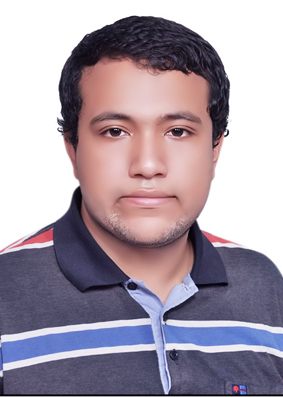
\includegraphics[width=0.6\linewidth]{moo}}};}
\begin{titlebox}[title={\color{white}المهمة}]\small\color{white}
أنا كخريج جديد من قسم الهندسة الكهربية أبحث عن فرص عمل تلبي احتياجاتي عن طريق عرض خدماتي مقابل مرتب مرض
\end{titlebox}%
}
};
\coordinate (sex) at ([yshift=-1cm]myname.south);
\path(sex) -- (myname);
\begin{scope}[remember picture, overlay, on background layer]
\fill [black] let \p1=(current page.north east), \p2=([xshift={-15pt-0.35\textwidth}]current page.north east),\p3=(myname.south),\p4=(sex) in (current page.north east) -- (\x1,\y3) -- 
(\x1,\y4)%(sex) 
-- (\x2,\y3) -- (\x2,\y2) -- cycle;
\end{scope}
\end{tikzpicture}
%
%\begin{tabular}{@{}rr@{}}
%\end{tabular}
\end{center}
%---------
\begin{titlebox}[title=معلومات شخصية]\renewcommand{\descriptionlabel}[1]{\color{blue} #1}%
\begin{description}[nosep,leftmargin=1.2em]%
\raggedleft\small%
\item[الاسم بالكامل:]\mbox{}\\ محمد \blackout{عبد المطلب إبراهيم عبد المطلب هاشم}
\item[محل الميلاد:]\mbox{}\\ \blackout{كوم النور، مركز ميت غمر، محافظة الدقهلة،} مصر
\item[تاريخ الميلاد:]\mbox{}\\22 من أغسطس، 1994
%\item[Nationality:]\mbox{}\\Egyptian
%\item[Marital status:]\mbox{}\\single
\item[للتواصل:]\mbox{}\\
\begin{itemize}[nosep,align=right,labelwidth=1.2em,labelsep=0.4em,leftmargin=1.6em]
	\item[\color{black}\faMobile*] \textenglish{+2 \blackout{01009968102}} \\ \textenglish{+2 \blackout{01063133400}}
	\item[\faGoogle] \resizebox{0.99\linewidth}{!}{\textenglish{{\fontfamily{lmtt}\selectfont m.hashim.666666\-@gmail.com}}}
	%\item[\color{blue}\faFacebook] {\ttfamily facebook.com/\blackout{themob911}} 
	\item[\color{blue}\faLinkedin]  \blackout{"Nothing"}
	\item[\color{green!50!black}\faWhatsapp] {+2 \blackout{01009968102}}
\end{itemize}
\end{description}
\end{titlebox}


\switchcolumn

\section[\large\faGraduationCap]{المؤهلات العلمية}
\subsection[\faSchool]{مدرسة \protect\blackout{كوم النور}
الثانوية (للبنين)
 \\ من سبتمبر 2010 إلى يونيو 2013}
	\begin{itemize}[nosep,leftmargin=*] 
		\item المجموع: 94.63\% \footnote{وفقا لنظام السنتين للثانوية العامة.}
	\end{itemize}
\subsection[\faUniversity]{كلية الهندسة - \protect\blackout{جامعة المنصورة} \\ \protect\blackout{من سبتمبر 2013 إلى يوليو 2019}}
	%\parbox[t]{0.5\linewidth}{%
	%\raggedright%
	\begin{itemize}[nosep,leftmargin=*] 
		\item قسم قوى وآلات كهربية \blackout{2014 - 2019}
		%\item Project grading: (Excellent)
		\item المجموع التراكمي : 71.79\% (بتقدير جيد)
	\end{itemize}
	%}%
%----------------------
\section[\faChartLine]{خبرات}
\subsection{دورات تدريبية}
%\subsection{دورة التحكم الآلي \LR{ِAutomation}  \\ من 28 يوليو حتى ---}
\begin{tcolorbox}[enhanced,bidibreakable,title={دورة التحكم الآلي \LR{ِAutomation}  \\ من 28 يوليو حتى ---}]
	\begin{itemize}[nosep,leftmargin=*,align=left]
		\item مركز التدريب: \LR{FATEC}
		\item عنوان المركز: شارع جيهان
		\item مدة التدريب: لمدة شهر تقريبًا.
		\item المهارات المكتسبة: 1) 
				\LR{Classic Control},
				2) \LR{Basic PLC}, 3) \LR{Motor drive}.
		%Experience Acquired: Learning 1) Classic control, 2) Basic PLC, 3) Motor drive.
	\end{itemize}
\end{tcolorbox}
%---------------
\subsection{تدريب ميداني}%
%\noindent \textit{This field is not yet well-filled, it needs more valuable information}
%\subsection{\protect\blackout{شركة عثمان أحمد عثمان للمواسير الخرسانية} | متدرَّب\\
%من يونيو 2017 إلى يوليو 2017}%%
\begin{tcolorbox}[enhanced,bidibreakable,title={\blackout{شركة عثمان أحمد عثمان للمواسير الخرسانية} | متدرَّب\\
من يونيو 2017 إلى يوليو 2017}]
	\begin{itemize}[nosep,leftmargin=*,align=left]
		\item المكان: وادي حوف، القاهرة.
		\item مدة التدريب: حوالي 20 يوم.
		\item الخبرات المكتسبة: معرفة مختصرة حول خطوط إنتاج المواسير والتحكم بها عن طريق 
			\LR{Automation}
	\end{itemize}
\end{tcolorbox}
%\subsection{\protect\blackout{محطة كهرباء طلخا} | متدرَّب\\ 
%من يولو 2016 إلى أغسطس 2016}%
	\begin{tcolorbox}[enhanced,bidibreakable,title={%
		\blackout{محطة كهرباء طلخا} |
		متدرب
		\\
		من يوليو 2016 إلى أغسطس 2016
	}]

	\begin{itemize}[nosep,leftmargin=*,align=left]
		\item المكان: مركز طلخا - محافظة الدقهلية 
		\item الخبرات المكتسبة: 
		\begin{itemize}[nosep,align=left,leftmargin=*]
			\item معرفة مختصرة حول كيفية توليد الطاقة بالبخار أو بالغاز أو بالدورات المركبة.
			%To know how plants actually produce electricity by vapor, gas or combined cycles. 
			\item معرفة مختصرة حول كيفية إدخال المحطات للشبكة ومن ثم نقل الطاقة للشبكة النقل العمومية.
			%To know how generators are synchronized with the grid whom energy is transmitted by.
		\end{itemize}
	\end{itemize}%
\end{tcolorbox}
%------------
\section[\faBullseye]{مهارات}
\subsection[\faLanguage]{مهارات لغوية}

\begin{cusbox}[title={اللغة العربية \hfill (لغة أم)},bidibreakable]
\end{cusbox}

\begin{cusbox}[title={اللغة الإنكليزية \footnotemark \hfill (\rating{{(3+2.5+1.8)/3}})},bidibreakable,before skip={\baselineskip}]\renewcommand{\thempfootnote}{\arabic{mpfootnote}}%
\setcounter{mpfootnote}{3}%
مهارة القراءة \hfill مقبول \rating{3}\\
مهارة الكتابة \hfill مقبول \rating{2.5} \\
مهارة التحدث والاستماع \hfill ضعيف \rating{1.8}
\end{cusbox}
\footnotetext{%
التقييمات المكتوبة هنا خاضعة لمعايير ذاتية. لم أخضع لاختبار حقيقي يقيس مستواي في اللغة
%These metrics are still based on my subjective criteria. No official test has been taken yet.
}
	%\item[Arabic (native)] \mbox{} \hfill (overall: Native) 
	%\item[English (in developpment)] \mbox{} \hfill (overall: good)\par
	%	\resizebox{\linewidth}{!}{\begin{tabular}{@{}lll@{}}
%		Reading & writing & speaking \\
%		\parbox{0.33\linewidth}{moderate} & \parbox{0.33\linewidth}{moderate} & \parbox{0.33\linewidth}%{poor}
%		\end{tabular}
%\end{description}}
\subsection[\faCogs]{المهارات الفنية}

%\begin{tabular}{@{}ll|ll@{}}
%Classic control & (in development) & PLC (basic \& advanced) & (in development) \\
%distribution & (in development) & SCADA & (in development) \\
%Motor drives & (in development) &    &
%\end{tabular}
\renewcommand{\thempfootnote}{\arabic{mpfootnote}}
\begin{cusbox}[title={\LR{Automation} \hfill (\rating{0})},bidibreakable,before skip={\baselineskip}]\renewcommand{\descriptionlabel}[1]{\jfflat #1}
\begin{description}[nosep]
\item[\LR{Classic control}]	\mbox{}{\textenglish{\unskip\nobreak\leaders\hbox{--}\hskip 4em plus 1fill}} \rating{2.45} \\ 
%	لأكون قادرا على استخدام المكونات المختلفة للتحكم في تشغيل وإيقاف المعدات والآلات.
أي تصميم دوائر كهربية للتحكم في تشغيل وإيقاف وتتابع تشغيل معدة ما أو عدة معدات باستخدام مكونات بدائية كالـ
\LR{Contactors} و 
\LR{Relays} و
\LR{Timers} 
.... وهكذا.
\item[\LR{PLC (مبتدئ)}] \mbox{}{\textenglish{\unskip\nobreak\leaders\hbox{--}\hskip 4em plus 1fill}} \rating{0.5}\\
%	وحدة التحكم القابلة للبرمجة تستخدم في التحكم في تشغيل وإيقاف المعدات بشكل 
يستخدم وحدة التحكم المنطقي القابل للبرمجة PLC في تنفيذ دوائر التحكم الأكثر تعقيدًا عن طريق برمجة الوحدة عن  لغة برمجة قد تكون 
\LR{Ladder Language} أو 
\LR{Statement programming} \hfill \LR{Self-Study}
\end{description}
\end{cusbox}

\subsection[\faLaptop]{مهارات الحاسوب}

\begin{cusbox}[title={لغات برمجة \hfill \rating{0}},bidibreakable,before skip={\baselineskip}]
\renewcommand{\descriptionlabel}[1]{\LR{\fontfamily{lmtt}\selectfont  #1}}%
\begin{description}[nosep]%
\item[MATLAB \& Simulink] \mbox{} \alongline \rating{2.5}
\item[\textenglish{\normalfont\LaTeX}] \mbox{} \alongline \rating{2.2}
\item[python] \mbox{} \alongline \rating{1}
\end{description}
\end{cusbox}

\begin{cusbox}[title={برامج CAD},bidibreakable,before skip={\baselineskip}]
\renewcommand{\descriptionlabel}[1]{\LR{\fontfamily{lmtt}\selectfont  #1}}%
\begin{description}[nosep]%
\item[TIA]\mbox{} \alongline \rating{1.2}
\end{description}
\end{cusbox}

\begin{cusbox}[title=أخرى,bidibreakable,before skip={\baselineskip}]
\renewcommand{\descriptionlabel}[1]{\LR{\fontfamily{lmtt}\selectfont  #1}}%
\begin{description}[nosep]%
\item[MS Word]\mbox{} \alongline \rating{3}
\item[MS Excel]\mbox{} \alongline \rating{2.2}
\end{description}
\end{cusbox}


\switchcolumn*
\tikz[remember picture]{\coordinate (last) at (0,0);}%
\setcounter{lastnum}{\value{page}}%
\end{paracol}
\vfill
\begin{tcolorbox}[
enhanced,interior hidden,frame code={
	\path (frame.north west) to [ornament=88] (frame.north east);
},left skip=4cm,right skip=4cm,left=0pt,right=0pt,
]
\small
هذا المسند قد كتب بلغة الـ
\LaTeX.
يمكنك الحصول على كود المصدر لقالب السيرة الذاتبة باللغتين (العربية والإنكليزية) مجانًا
واستعمالها كما تشاء عن طريق الموقع الآتي:

\textenglish{{\fontfamily{lmtt}\selectfont www.kosomak.com}}

وإذا أردت تنسيق السيرة الذاتية على هذا النحو بالنيابة عنك فيمكن التواصل معي عبر وسائل التواصل المختلفة 
المذكورة أعلاه

\mbox{} \hfill \begin{varwidth}{5cm} \raggedright  مع تحياتي \\ محمد عبد المطلب هاشم \end{varwidth}
\end{tcolorbox}
\end{document}